\documentclass[10pt]{beamer}

\usetheme[progressbar=frametitle]{metropolis}
\usepackage{ctex}
\usepackage{appendixnumberbeamer}

\usepackage{booktabs}
\usepackage[scale=2]{ccicons}

\usepackage{pgfplots}
\usepgfplotslibrary{dateplot}

\usepackage{xspace}
\newcommand{\themename}{\textbf{\textsc{metropolis}}\xspace}
\usepackage{subfig}
\usepackage[ruled,vlined,linesnumbered]{algorithm2e}
\renewcommand{\algorithmcfname}{算法} %针对 algorithm2e 宏包
\usepackage{tikz}
\usepackage{pgfplots}
\usetikzlibrary{positioning}

\graphicspath{{fig/}}

\title{基于RGB-D图像的三维物体识别算法的研究与实现}
% \subtitle{A modern beamer theme}
% \date{\today}
\author{李勇奇\hskip12pt 指导教师:陈启军}
\institute{同济大学,控制科学与工程系}
% \titlegraphic{\hfill
\includegraphics[height=1.5cm]{tongji-whole-logo}}
\begin{document}

\maketitle

\begin{frame}{Table of contents}
  \label{contents}
  \setbeamertemplate{section in toc}[sections numbered]
  \tableofcontents[hideallsubsections]
\end{frame}

\section{Introduction}

\begin{frame}[fragile]{Problem}
  \begin{center}
  \begin{tikzpicture}
    \uncover<2->{\node[anchor=south west] (left-image) at (0,0) {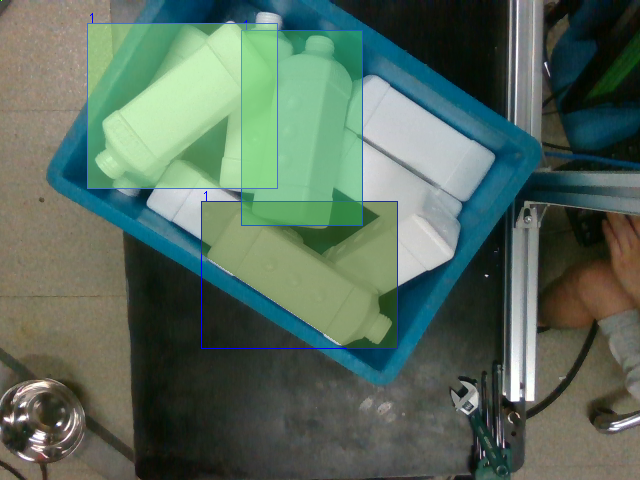
\includegraphics[height=5cm]{2d-detection-results}};}
    \uncover<3->{\node[right=0.2of left-image] (right-image) {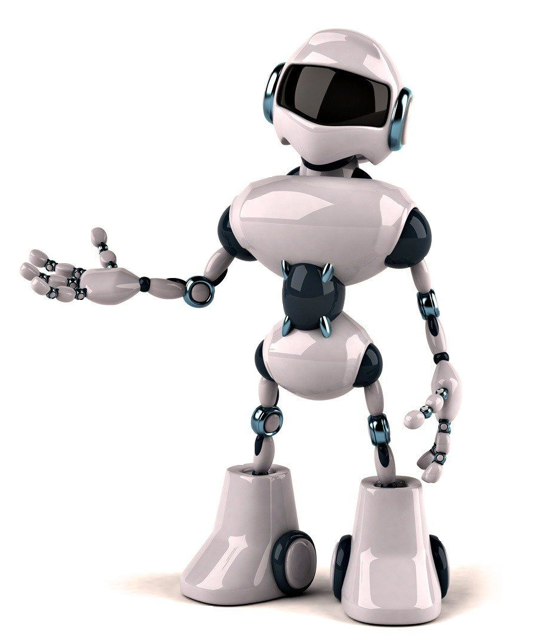
\includegraphics[height=5cm]{robot}};}
    \uncover<2->{\node[align=center, font={\Large\bfseries}, above=0.2of left-image] {2D Detection};}
    \uncover<3->{\node[align=center, font={\Large\bfseries}, above=0.2of right-image] {Where to pick?};}
    \only<4->{\node[draw=blue, fill=blue!40!white,fill opacity=0.6, align=center, font={\Huge\bfseries}, text=black] at (0.5\textwidth, 0.5\textheight-40) {Robotics has a\\Perception Problem!};}
  \end{tikzpicture}
  \end{center}
\end{frame}

\begin{frame}[fragile]{3D Detection}
  \begin{center}
  \begin{tikzpicture}
    \uncover<2->{\node[anchor=south west] (lefttop-image) at (0,0) {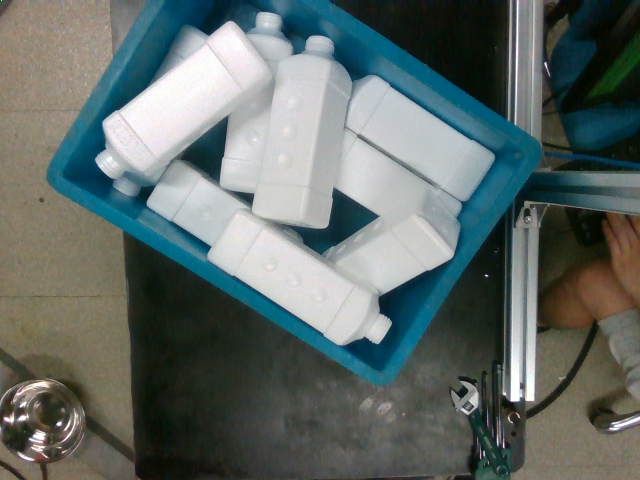
\includegraphics[width=4cm]{color1}};}
    \uncover<2->{\node[below=0.2of lefttop-image] (leftbottom-image) {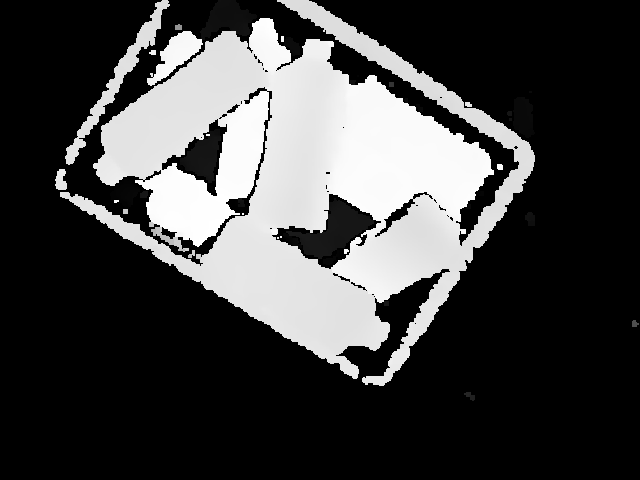
\includegraphics[width=4cm]{depth1}};}
    \node[below right=-.2of lefttop-image] (middle-node) {};
    \uncover<3->{\node[right=1.5of middle-node] (right-image) {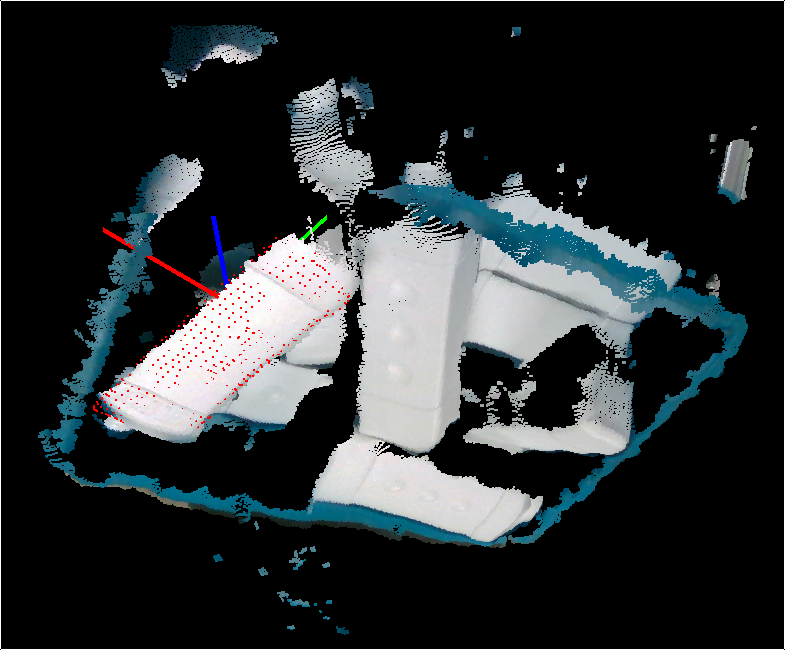
\includegraphics[width=4cm]{3d-detection-results}};}
    \uncover<3->{\draw[very thick,->] (middle-node) to (right-image.west);}
    \uncover<2->{\node[align=center, above=0.1of lefttop-image] {RGB Image};}
    \uncover<2->{\node[align=center, below=0.1of leftbottom-image] {Depth Map};}
    \uncover<3->{\node[align=center, above=0.1of right-image] {3D Detection Results};}
  \end{tikzpicture}
  \end{center}
\end{frame}

\section{Dual RGB-D Camera}

\begin{frame}[fragile]{Problem \& Key}
  \uncover<2-> {{\bf Problem:} SR300相机对反光物体在某些角度下深度信息有严重的缺失}
  \uncover<2-> {
  \begin{figure}
    \centering
    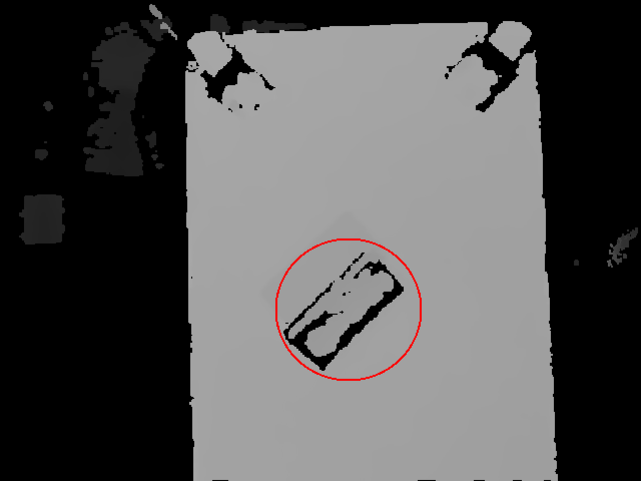
\includegraphics[width=3.5cm]{left_depth}
  \end{figure}
  }
  \uncover<3-> {{\bf Key:} 改变相机的拍摄角度}
  \uncover<3-> {
  \begin{figure}
    \centering
    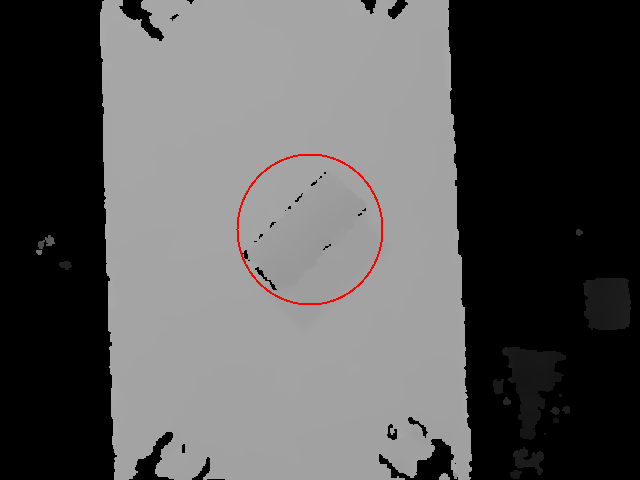
\includegraphics[width=3.5cm]{right_depth}
  \end{figure}
  }
\end{frame}

\begin{frame}[fragile]{Structure of Dual RGB-D Camera}
  \begin{tikzpicture}
    \uncover<2->{\node[anchor=north west] (left-image) at (0,0) {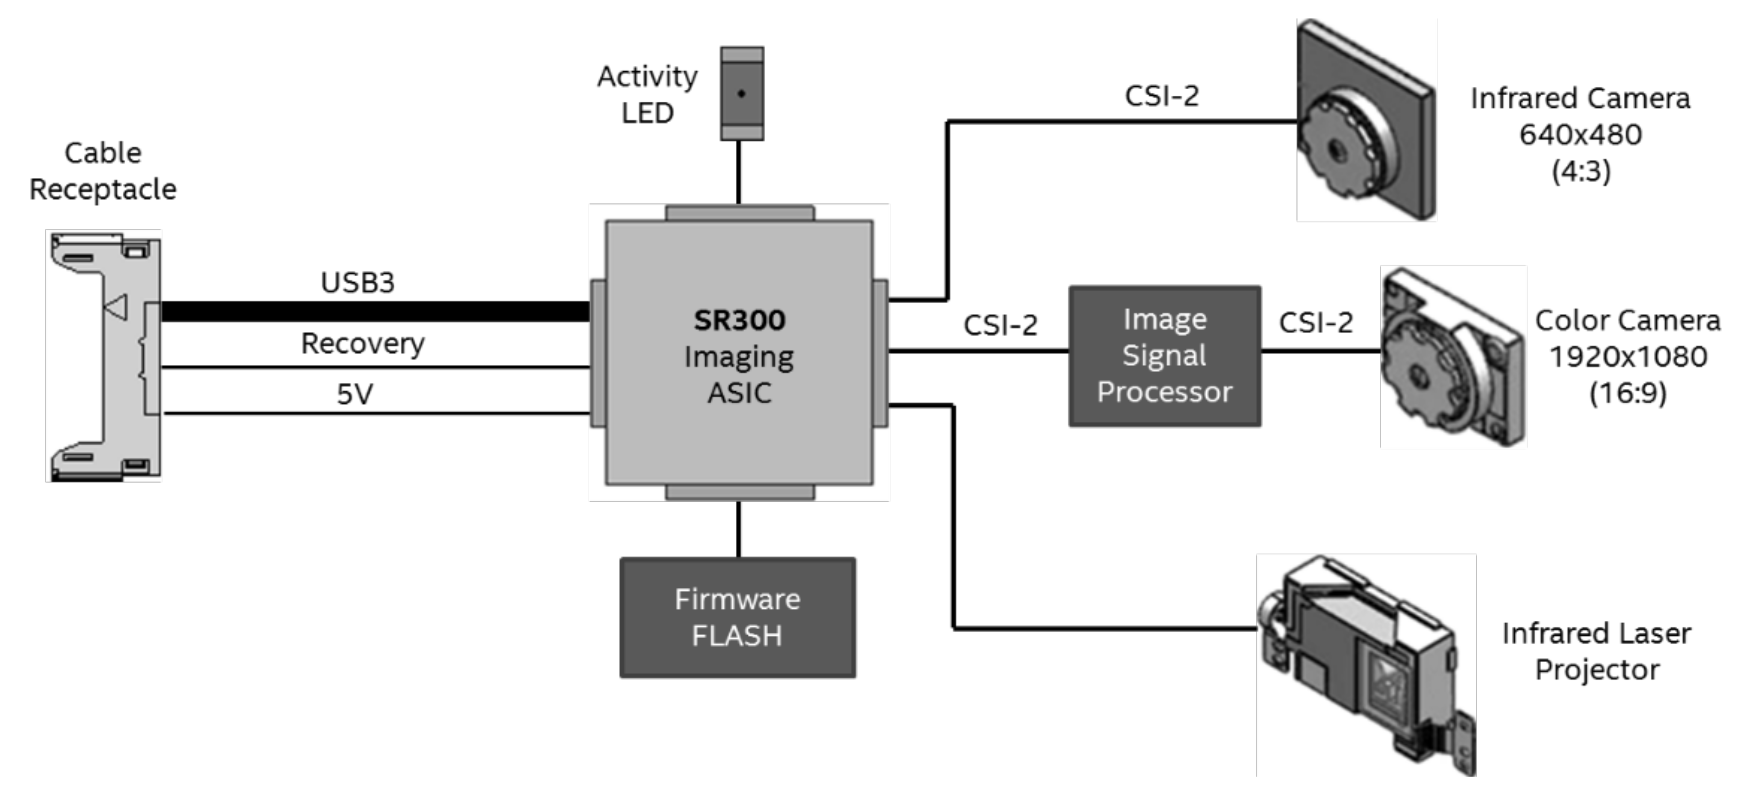
\includegraphics[width=4cm]{dual_rgbd}};}
    \uncover<3->{\node[right=0.2of left-image] (right-image) {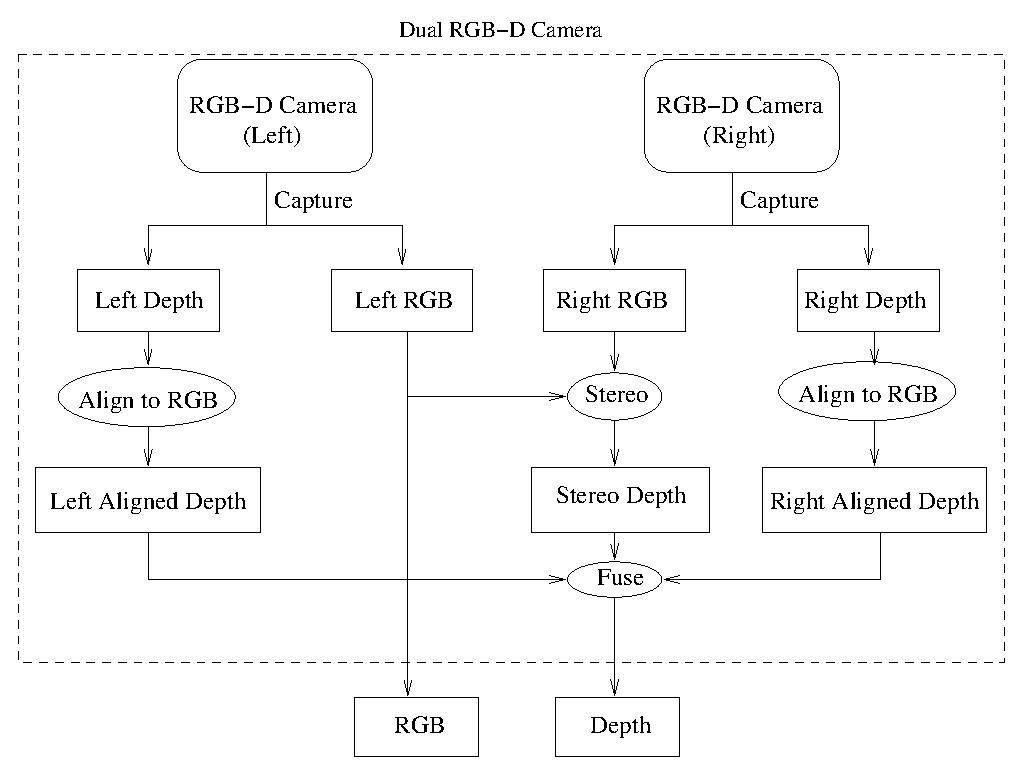
\includegraphics[width=6cm]{dual_rgbd_struct}};}
    \uncover<2->{\node[align=center, below=0.1of left-image] {对偶RGB-D相机物理结构};}
    \uncover<3->{\node[align=center, below=0.1of right-image] {对偶RGB-D相机内部原理图};}
  \end{tikzpicture}
\end{frame}

\begin{frame}[fragile]{Implementation}
  \vskip0.2cm
  \begin{columns}
    \begin{column}{0.4\textwidth}
      \begin{itemize}
        \item<3-> 将深度图与彩色图对齐
        \item<4-> 通过双目匹配算法(ELAS)形成一张新的深度图
        \item<5-> 融合三张深度图
      \end{itemize}
    \end{column}
    \uncover<2->{
    \begin{column}{0.49\textwidth}
      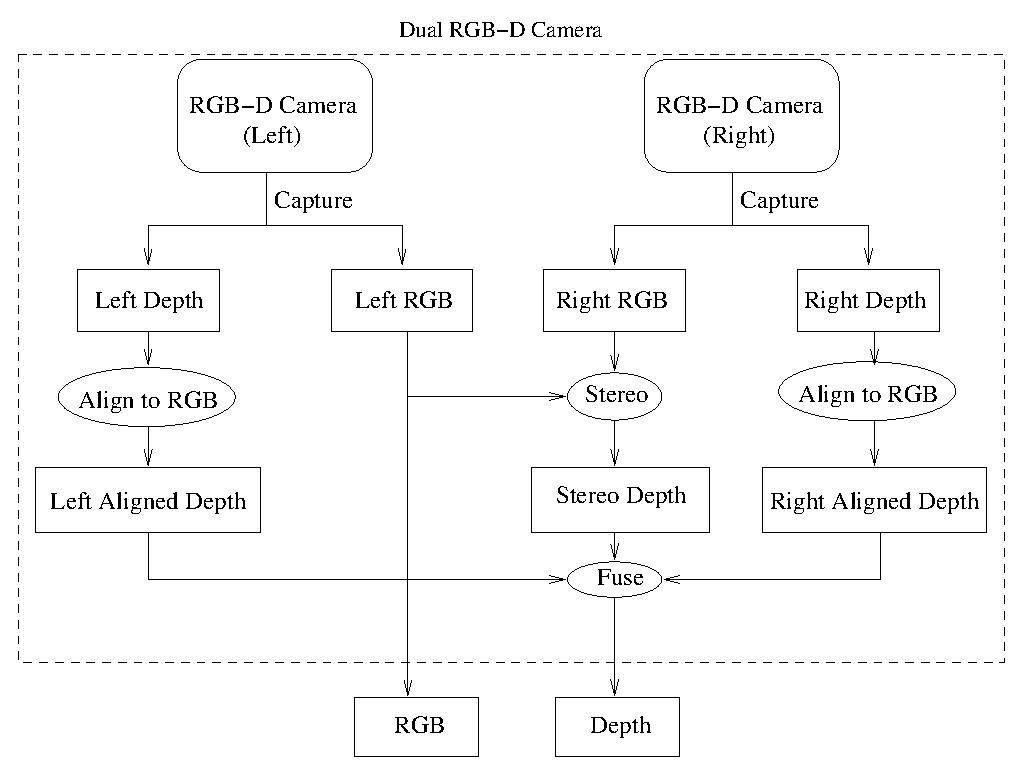
\includegraphics[width=6cm]{dual_rgbd_struct}
    \end{column}
    }
  \end{columns}
  \vfill
  \begin{center}
  \begin{tikzpicture}
    \uncover<6->{
      \node (upper) {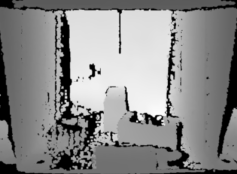
\includegraphics[height=1.8cm]{upper-depth}};
      \node [right=0.2 of upper] (lower) {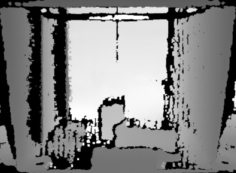
\includegraphics[height=1.8cm]{lower-depth}};
      \node [right=0.2 of lower] (stereo) {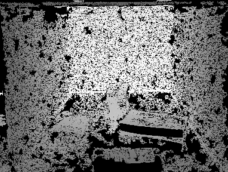
\includegraphics[height=1.8cm]{stereo-depth}};
      \node [right=0.2 of stereo] (fuse) {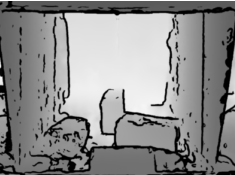
\includegraphics[height=1.8cm]{fuse-depth}};
      \node [below=0 of upper, font={\tiny}] {Upper Depth};
      \node [below=0 of lower, font={\tiny}] {Lower Depth};
      \node [below=0 of stereo, font={\tiny}] {Stereo Depth};
      \node [below=0 of fuse, font={\tiny}] {Fuse Depth};}
  \end{tikzpicture}
  \end{center}
\end{frame}

\begin{frame}[fragile]{Experiment \& Results}
  \begin{tikzpicture}
    \uncover<2->{
      \node (fillrate) {
        \begin{tikzpicture}[scale=0.4]
          \begin{axis}[xlabel=$d$ (m), ylabel=Fill Rate (\%)]
            \addplot[smooth, mark=*, blue] plot coordinates {
              (0.2, 97)
              (0.3, 98.2)
              (0.4, 98)
              (0.5, 96)
              (0.6, 94)
              (0.7, 92)
              (0.8, 90)
              (0.9, 88)
              (1.0, 87)
              (1.1, 84)
              (1.2, 80)
            };
            \addlegendentry{Dual RGB-D}
            \addplot[smooth, mark=x, red] plot coordinates {
              (0.2, 94)
              (0.3, 93.5)
              (0.4, 93.1)
              (0.5, 91.3)
              (0.6, 90.3)
              (0.7, 89)
              (0.8, 87.2)
              (0.9, 85)
              (1.0, 81)
              (1.1, 78)
              (1.2, 74)
            };
            \addlegendentry{SR300}
          \end{axis}
        \end{tikzpicture}
      };
      \node [below=0.1 of fillrate] {$\frac{M'}{M} \times 100\%$};
    }
    \uncover<3->{
      \node [right =0.1 of fillrate] (precision) {
        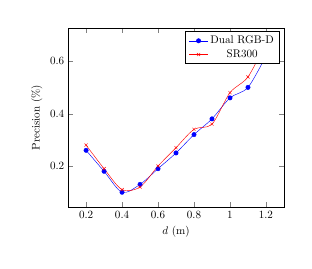
\begin{tikzpicture}[scale=0.4]
          \begin{axis}[xlabel=$d$ (m), ylabel=Precision (\%)]
            \addplot[smooth, mark=*, blue] plot coordinates {
              (0.2, 0.26)
              (0.3, 0.18)
              (0.4, 0.10)
              (0.5, 0.13)
              (0.6, 0.19)
              (0.7, 0.25)
              (0.8, 0.32) 
              (0.9, 0.38)
              (1.0, 0.46)
              (1.1, 0.50)
              (1.2, 0.62)
            };
            \addlegendentry{Dual RGB-D}
            \addplot[smooth, mark=x, red] plot coordinates {
              (0.2, 0.28)
              (0.3, 0.19)
              (0.4, 0.11)
              (0.5, 0.12)
              (0.6, 0.20)
              (0.7, 0.27)
              (0.8, 0.34)
              (0.9, 0.36)
              (1.0, 0.48)
              (1.1, 0.54)
              (1.2, 0.67)
            };
            \addlegendentry{SR300}
          \end{axis}
        \end{tikzpicture}
      };
      \node [below=0.1 of precision] {$\frac{|\hat{d}-d|}{d} \times 100\%$};
    }
    \uncover<4->{
      \node [right =0.1 of precision] (noise) {
        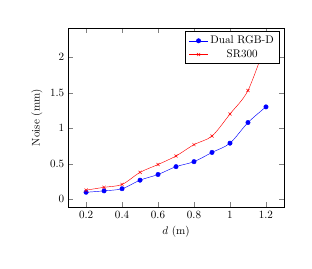
\begin{tikzpicture}[scale=0.4]
          \begin{axis}[xlabel=$d$ (m), ylabel=Noise (mm)]
            \addplot[smooth, mark=*, blue] plot coordinates {
              (0.2, 0.1)
              (0.3, 0.12)
              (0.4, 0.15)
              (0.5, 0.27)
              (0.6, 0.35)
              (0.7, 0.46)
              (0.8, 0.53)
              (0.9, 0.66)
              (1.0, 0.79)
              (1.1, 1.08)
              (1.2, 1.3)
            };
            \addlegendentry{Dual RGB-D}
            \addplot[smooth, mark=x, red] plot coordinates {
              (0.2, 0.13)
              (0.3, 0.17)
              (0.4, 0.21)
              (0.5, 0.38)
              (0.6, 0.49)
              (0.7, 0.61)
              (0.8, 0.77)
              (0.9, 0.89)
              (1.0, 1.2)
              (1.1, 1.53)
              (1.2, 2.2)
            };
            \addlegendentry{SR300}
          \end{axis}
        \end{tikzpicture}
      };
      \node [below=0.1 of noise] {$\sqrt{\frac{1}{N}\sum_{i=1}^N{\delta_i^2}}$};
    }
  \end{tikzpicture}
\end{frame}

\section{3D-MRAI Algorithm}

\begin{frame}[fragile]{3D-MRAI}
  \begin{center}
  \uncover<2->{
    3D-MRAI (3D Mask R-CNN with Angle-fixed-4PCS and ICP)
    \vskip0.5cm
  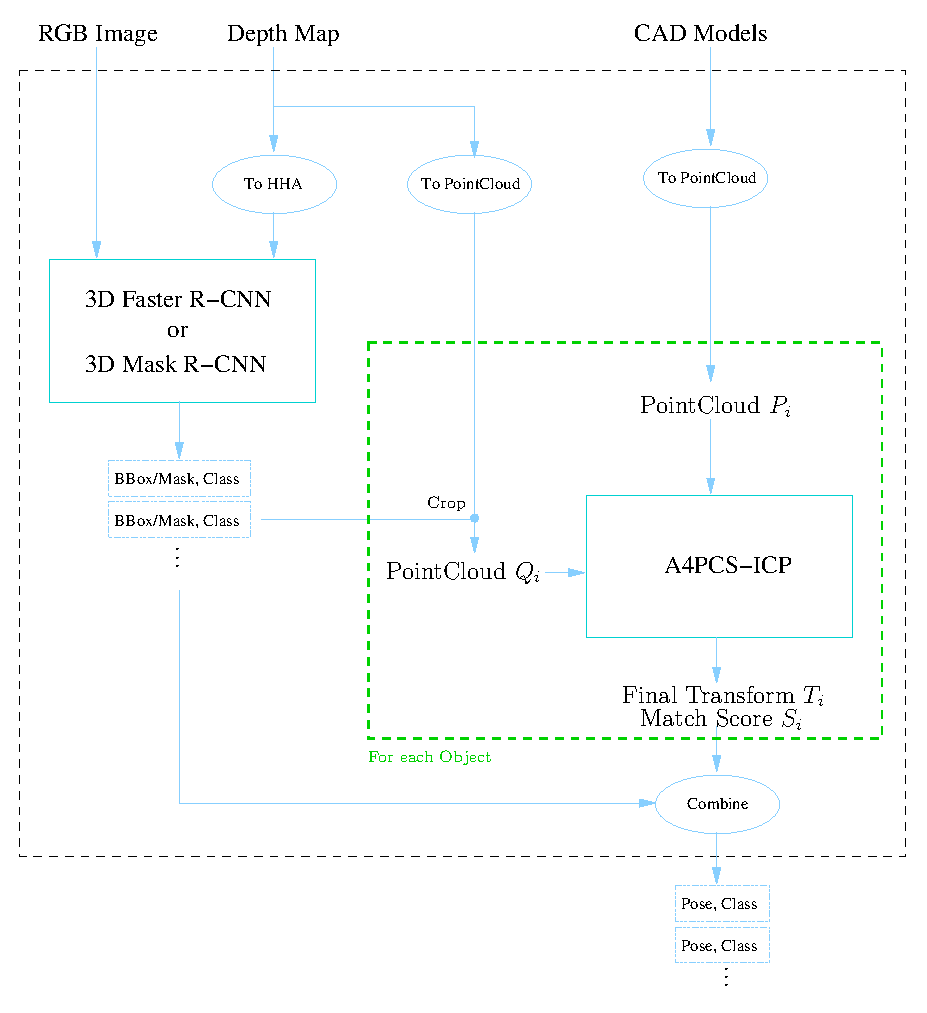
\includegraphics[height=0.8\textheight]{detect-pose}
  }
  \end{center}
\end{frame}

\subsection{Detection Module}
\begin{frame}[fragile]{Detection Module}
  \begin{center}
  \begin{tikzpicture}
    \uncover<2->{\node (left-image) at (0,0) {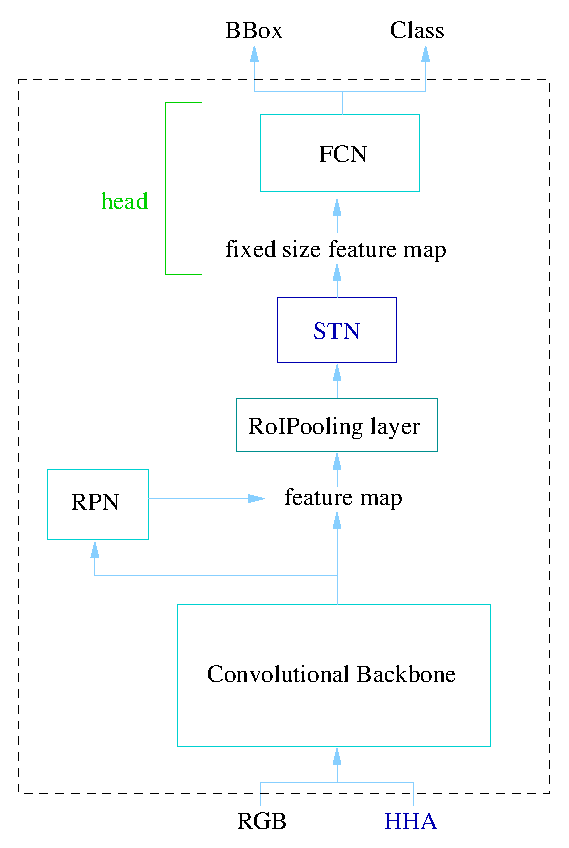
\includegraphics[height=6cm]{faster_rcnn_module}};}
    \uncover<2->{\node [below=0.1of left-image] {Based on Faster R-CNN};}
    \uncover<3->{\node [right=0.5of left-image] (right-image) {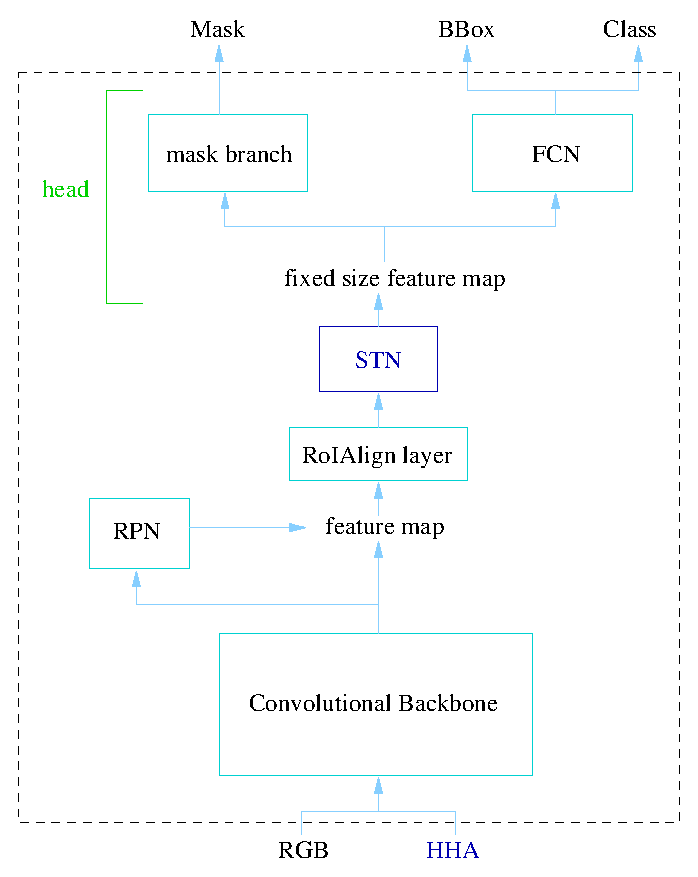
\includegraphics[height=6cm]{mask_rcnn_module}};}
    \uncover<3->{\node [below=0.1of right-image] {Based on Mask R-CNN};}
  \end{tikzpicture}
  \end{center}
\end{frame}

\begin{frame}[fragile]{Mask R-CNN Module}
  \begin{center}
  \begin{tikzpicture}
    \uncover<2->{\node (left-image) at (0,0) {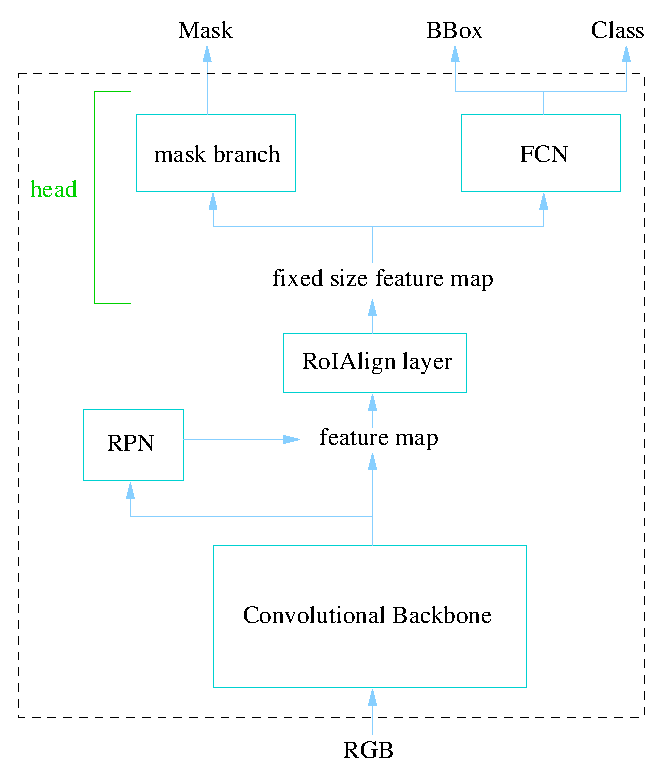
\includegraphics[height=5cm]{mask_rcnn}};}
    \uncover<2->{\node [below=0.1of left-image] {Original Mask R-CNN};}
    \uncover<3->{\node [right=0.5of left-image] (right-image) {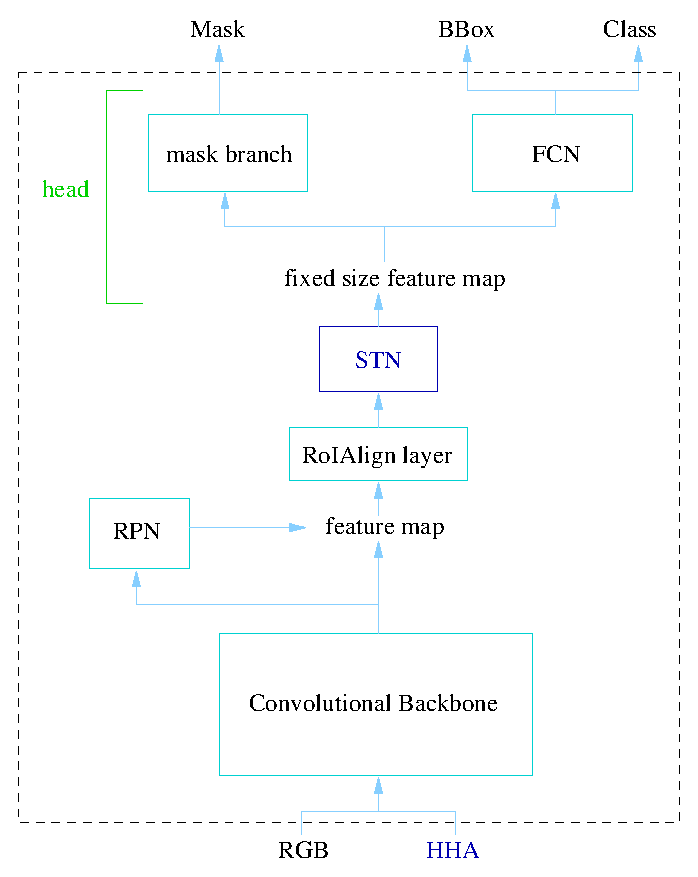
\includegraphics[height=5cm]{mask_rcnn_module}};}
    \uncover<3->{\node [below=0.1of right-image] {Mask R-CNN Detection Module};}
  \end{tikzpicture}
  \end{center}
  \vskip-12pt
  \begin{itemize}
  \item<4-> 引入HHA,有效利用三维信息,解决原算法难以检测纹理缺少的物体
  \item<5-> 在网络中增加STN(Spatial Transformer Network),使得提取的特征具有旋转不变性,增加了算法检测准确度
  \end{itemize}
\end{frame}

\begin{frame}
  \frametitle{Detection Module}
  \begin{center}
    \uncover<2->{
    \begin{tikzpicture}
      \node (hd) {
\includegraphics[width=2.5cm]{disparity_frame}};
      \node [below=0.1of hd, font={\tiny}] {Horizontal disparity frame};
      \node [right=0.2of hd] (hg) {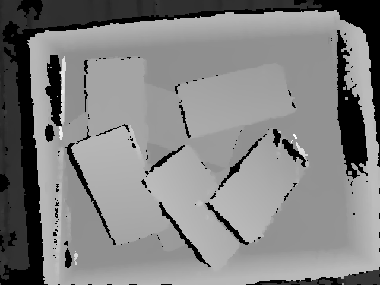
\includegraphics[width=2.5cm]{height_frame}};
      \node [below=0.1of hg, font={\tiny}] {Height above ground frame};
      \node [right=0.2of hg] (ag) {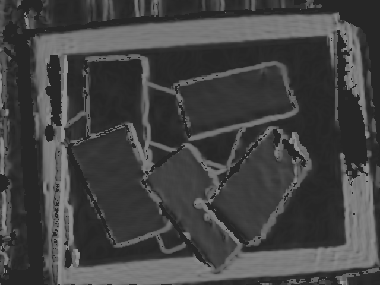
\includegraphics[width=2.5cm]{angle_frame}};
      \node [below=0.1of ag, font={\tiny}] {Angle with gravity frame};
      \node [right=0.2of ag] (hha) {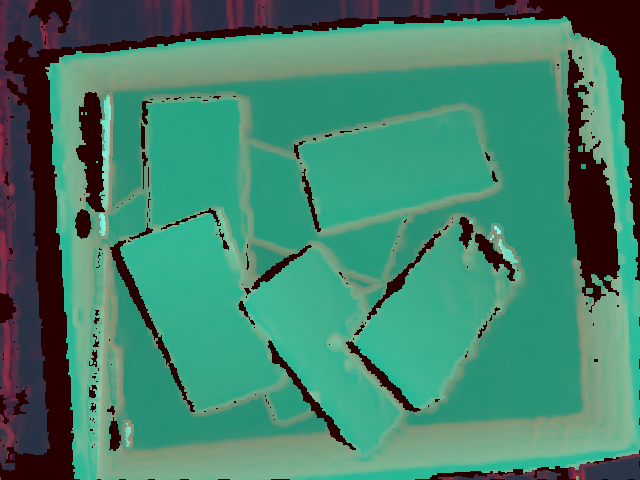
\includegraphics[width=2.5cm]{hha_frame}};
      \node [below=0.1of hha, font={\tiny}] {HHA frame};
    \end{tikzpicture}
    }
  \end{center}
  \vfill
  \begin{center}
    \uncover<3->{
    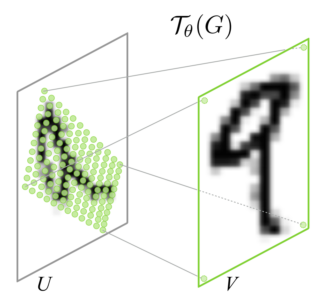
\includegraphics[width=4.5cm]{grid-generator}
    }
  \end{center}
\end{frame}

\begin{frame}{Detection Module Results}
  \uncover<2->{
\begin{table}[ht]
  \centering
  \caption{APC数据集上的精确度}
  \resizebox{10cm}{!}{
    \begin{tabular}{cccccc}
      \toprule
      &input&output&$AP$&$AP_{0.5}$&$AP_{0.75}$ \\
      \midrule
      Faster R-CNN&RGB&bbox&33.26&56.29&34.03 \\
      \bf{Our method(based on Faster R-CNN)}&RGB+HHA&bbox&\bf{34.55}&\bf{57.99}&\bf{34.69} \\
      Mask R-CNN&RGB&mask&32.34&55.78&33.12 \\
      \bf{Our method(based on Mask R-CNN)}&RGB+HHA&mask&\bf{33.94}&\bf{56.45}&\bf{33.99} \\
      \bottomrule
    \end{tabular}}
  \label{tab:ap1}
\end{table}
  }
  \uncover<3->{
\begin{table}[ht]
  \centering
  \caption{workpiece数据集上的精确度}
  \resizebox{10cm}{!}{
    \begin{tabular}{cccccc}
      \toprule
      &input&output&$AP$&$AP_{0.5}$&$AP_{0.75}$ \\
      \midrule
      Faster R-CNN&RGB&bbox&18.78&37.49&19.46 \\
      \bf{Our method(based on Faster R-CNN)}&RGB+HHA&bbox&\bf{32.39}&\bf{56.37}&\bf{33.54} \\
      Mask R-CNN&RGB&mask&16.12&35.95&18.74 \\
      \bf{Our method(based on Mask R-CNN)}&RGB+HHA&mask&\bf{30.98}&\bf{53.74}&\bf{32.19} \\
      \bottomrule
    \end{tabular}}
  \label{tab:ap2}
\end{table}
  }
\end{frame}

\subsection{Matching Module}
\begin{frame}{Matching Module}
  \begin{columns}
    \begin{column}{0.4\textwidth}
      \begin{itemize}
      \item<3-> 去除4PCS算法中角度不相等的基,减少了算法运算时间
      \item<4-> 通过增加滤波和ICP算法,增加了匹配精度
      \end{itemize}
    \end{column}
    \uncover<2->{
    \begin{column}{0.58\textwidth}
      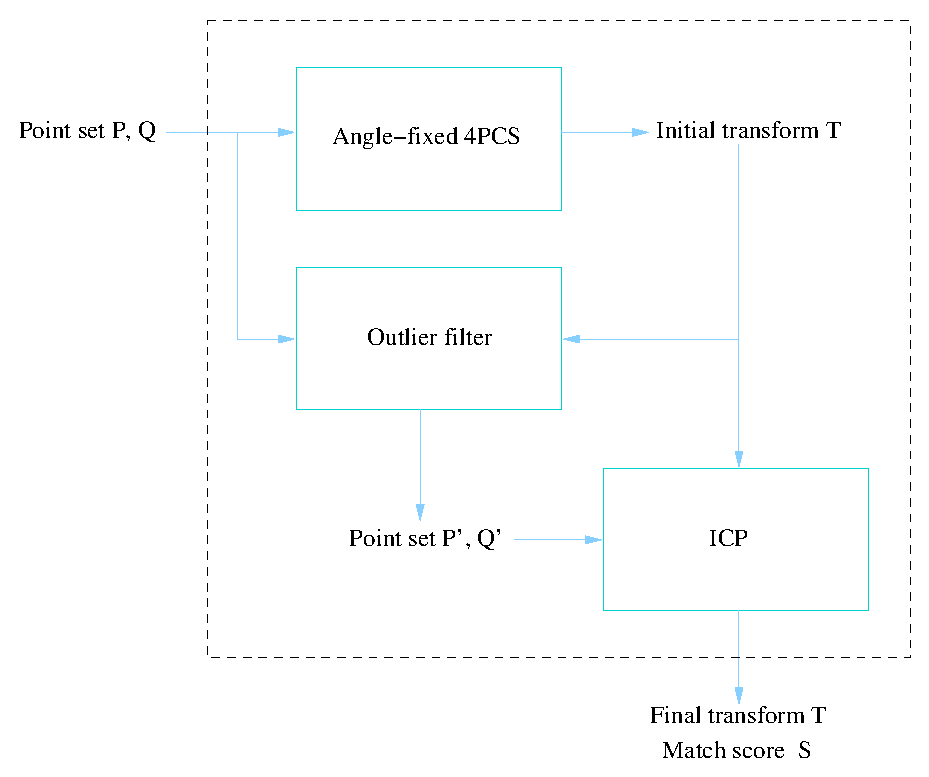
\includegraphics[width=6cm]{4pcs-pe}
    \end{column}}
  \end{columns}
\end{frame}

\begin{frame}{Matching Module}
  \begin{center}
  \begin{tikzpicture}
    \uncover<2->{
      \node (pic) {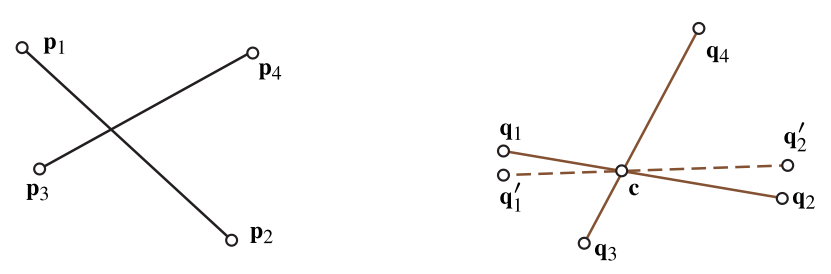
\includegraphics[width=7cm]{4pcs-flaw}};
      \node [below=0.1of pic] {4PCS存在的问题};
    }
  \end{tikzpicture}
  \vfill
  \begin{tikzpicture}
    \uncover<3->{
      \node (object) {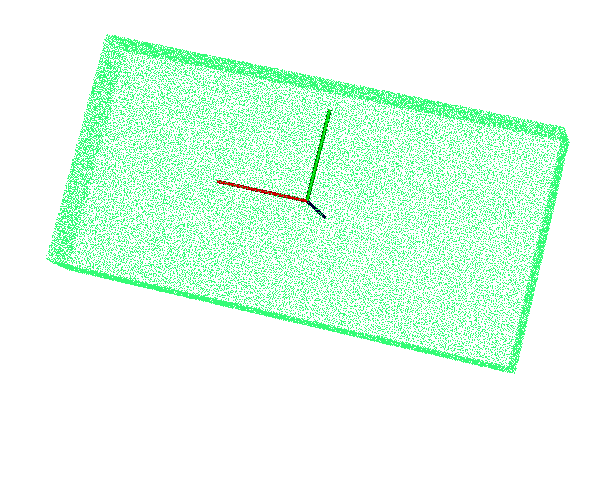
\includegraphics[height=3cm]{object-cloud}};
      \node[right =2 of object] (target) {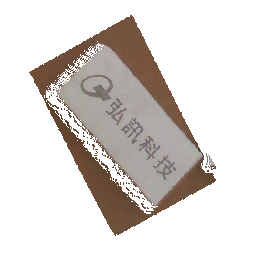
\includegraphics[height=3cm]{target-cloud}}; 
      \node [below=0.1of object] {目标3D模型转化的点云};
      \node [below=0.1of target] {从BBox裁剪得到的点云};
    }
  \end{tikzpicture}
  \end{center}
\end{frame}


\begin{frame}{Matching Module Results}
  \begin{center}
  \uncover<2->{
  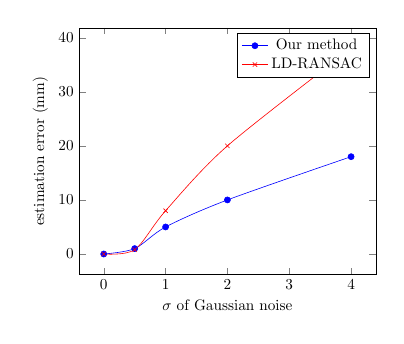
\begin{tikzpicture}[scale=0.55]
    \begin{axis}[xlabel=$\sigma$ of Gaussian noise, ylabel=estimation error (mm)]
      \addplot[smooth, mark=*, blue] plot coordinates {
        (0, 0)
        (0.5,1)
        (1, 5)
        (2, 10)
        (4, 18)
      };
      \addlegendentry{Our method}
      \addplot[smooth, mark=x, red] plot coordinates {
        (0, 0)
        (0.5,0.8)
        (1, 8)
        (2, 20)
        (4, 38)
      };
      \addlegendentry{LD-RANSAC}
    \end{axis}
  \end{tikzpicture}
  }
  \hskip1cm
  \uncover<3->{
  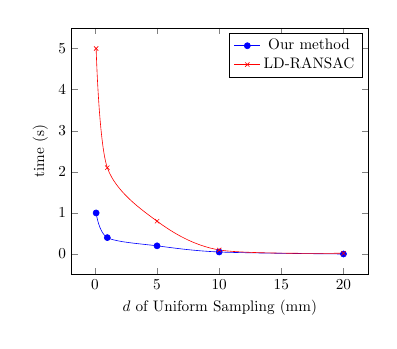
\begin{tikzpicture}[scale=0.55]
    \begin{axis}[xlabel=$d$ of Uniform Sampling (mm), ylabel=time (s)]
      \addplot[smooth, mark=*, blue] plot coordinates {
        (0.1, 1)
        (1,0.4)
        (5, 0.2)
        (10, 0.05)
        (20, 0.001)
      };
      \addlegendentry{Our method}
      \addplot[smooth, mark=x, red] plot coordinates {
        (0.1, 5)
        (1,2.1)
        (5, 0.8)
        (10, 0.1)
        (20, 0.02)
      };
      \addlegendentry{LD-RANSAC}
    \end{axis}
  \end{tikzpicture}
  }
  \vfill
  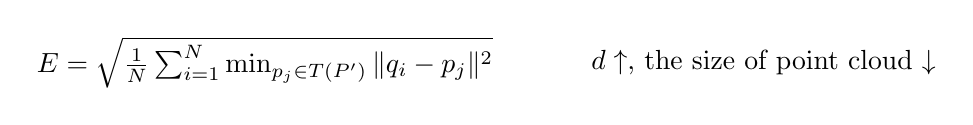
\begin{tikzpicture}
    \uncover<2->{
      \node (error) {$E = \sqrt{\frac{1}{N}\sum_{i=1}^{N}{\min_{p_j\in T(P')}\|{q_i-p_j}\|^2}}$};
    }
    \uncover<3->{
      \node[right =1. of error] {$d \uparrow$, the size of point cloud $\downarrow$};
  }
  \end{tikzpicture}
  \end{center}
\end{frame}

\begin{frame}{Combine Everything}
  \begin{columns}
    \uncover<2->{
    \begin{column}{0.49\textwidth}
\scalebox{.75}{
\begin{algorithm}[H]
  \caption{3D-MRAI算法}
  \KwIn{RGB Image $I$, Depth Map $D$, CAD Models $M$}
  \KwOut{Set of Pose and Class $Res$}
  $Res\leftarrow \varnothing$\;
  $P\leftarrow \varnothing$\;
  \ForAll {$M_i\in M$} {
    $P\leftarrow \left\{P, CAD2PointCloud(M_i)\right\}$\;
  }
  $H = Depth2HHA(D)$\;
  $Q = Depth2PointCloud(D)$\;
  $Mask, Class \leftarrow DetectModule(I, H)$\;
  \ForAll {$m_i\in Mask, c_i\in Class$} {
    $Q_i \leftarrow Crop(Q, m_i)$\;
    $P_i \leftarrow P(c_i)$\;
    $T_i,S_i\leftarrow MatchModule(P_i, Q_i)$\;
    \If {$S_i > S_{min}$} {
      $Res\leftarrow \left\{Res, \left[T_i, c_i\right]\right\}$\;
    }
  }
  \Return $Res$
\end{algorithm}}
    \end{column}
    }
    \begin{column}{0.49\textwidth}
      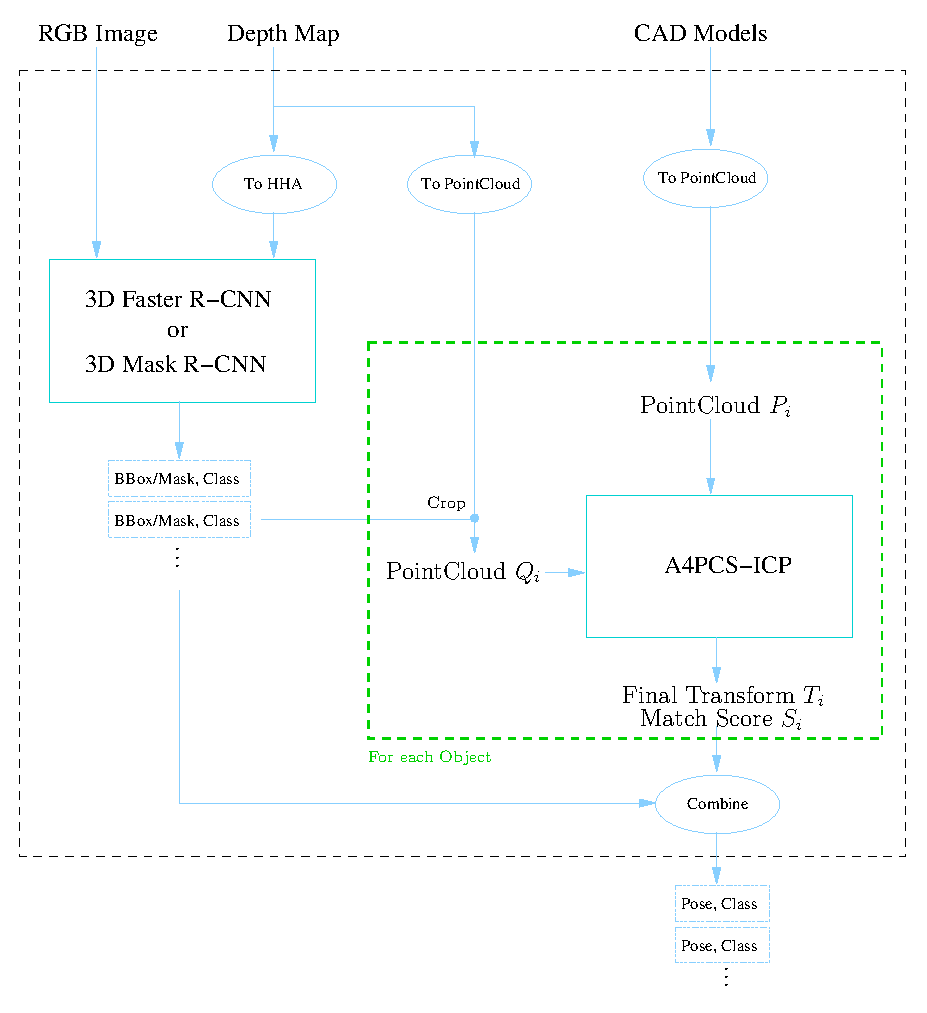
\includegraphics[width=5.5cm]{detect-pose}
    \end{column}
  \end{columns}
\end{frame}

\begin{frame}{3D-MRAI Results}
  \begin{center}
  \uncover<2-> {
  \begin{tikzpicture}
    \node (res1) {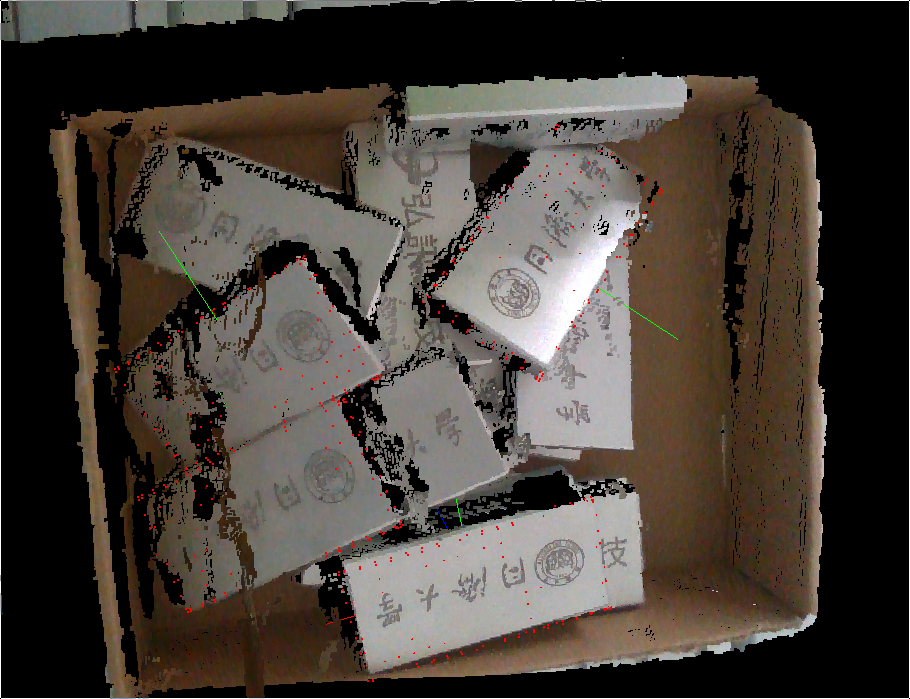
\includegraphics[height=2cm]{3dmrai-res1}};
    \node [right=0.2 of res1] (res2) {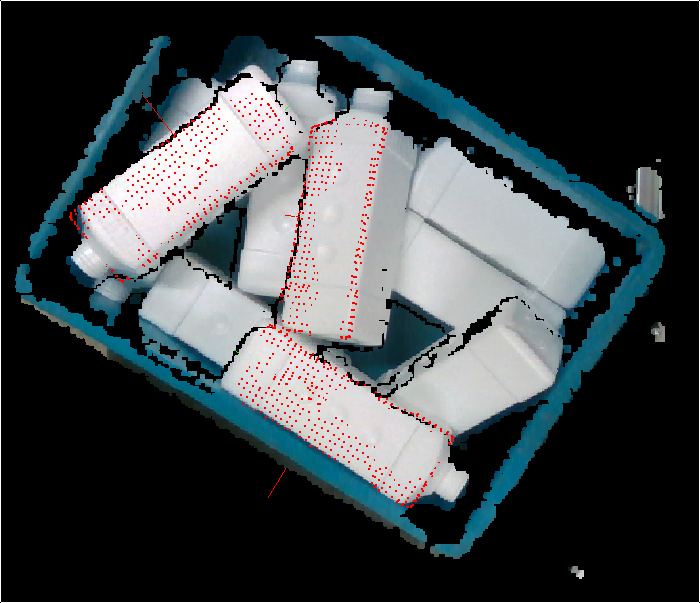
\includegraphics[height=2cm]{3dmrai-res2}};
    \node [right=0.2 of res2] (res3) {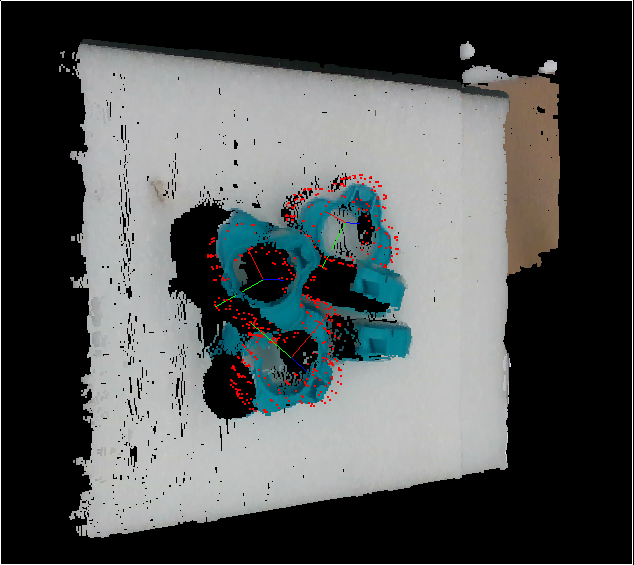
\includegraphics[height=2cm]{3dmrai-res3}};
  \end{tikzpicture}
  }
  \end{center}
  \vskip1pt
  \uncover<3->{
  \resizebox{10cm}{!}{
  \begin{tabular}{ccccccc}
    \toprule
    $k_m[\%]$&5&7&9&11&13&15\\
    \midrule
    Hinterstorisser et al.&75.63& 83.84& 89.13& 93.48& 96.83&98.12\\
    \bf{3D-MRAI}&95.12& 97.35& 98.10& 98.69& 99.22& 100.00\\
    \bottomrule
  \end{tabular}}
  }
  \vskip6pt
  \begin{columns}
    \uncover<5->{
    \begin{column}{0.49\textwidth}
      \begin{equation*}
        m = {\underset{\mathbf{x}\in M}{avg}} \; {\parallel (R\mathbf{x}+t) - (\tilde{R}\mathbf{x}+\tilde{t})\parallel}
      \end{equation*}
      如果$m < k_md$,算法输出位姿正确
    \end{column}}
    \uncover<4->{
      \begin{column}{0.49\textwidth}
        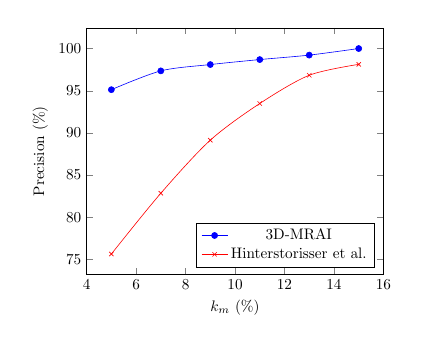
\begin{tikzpicture}[scale=0.55]
          \begin{axis}[xlabel=$k_m$ (\%),
            ylabel=Precision (\%),
            legend pos=south east,]
            \addplot[smooth, mark=*, blue] plot coordinates {
              (5, 95.12)
              (7, 97.35)
              (9, 98.1)
              (11, 98.69)
              (13, 99.22)
              (15, 100.00)
            };
            \addplot[smooth, mark=x, red] plot coordinates {
              (5, 75.63)
              (7, 82.84)
              (9, 89.13)
              (11, 93.48)
              (13, 96.83)
              (15, 98.12)
            };
            \legend{3D-MRAI,Hinterstorisser et al.}
          \end{axis}
        \end{tikzpicture}
      \end{column}}
  \end{columns}
\end{frame}

\section{Application: Bin-picking}
\begin{frame}
  \frametitle{System Structure}
  \begin{tikzpicture}
    \uncover<2->{\node (left-image) at (0,0) {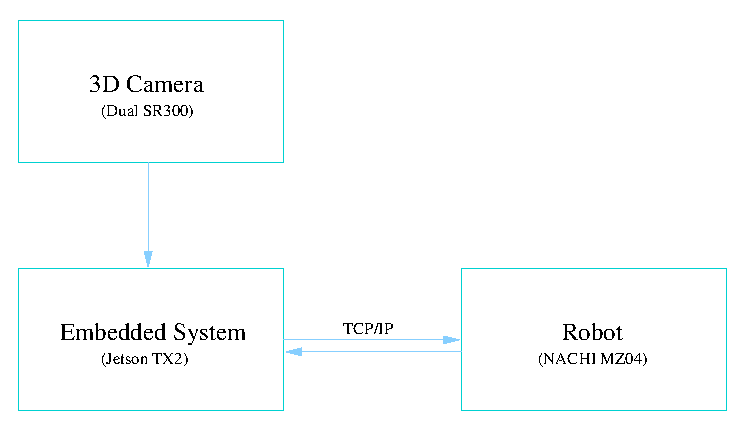
\includegraphics[width=6cm]{hardware-sys}};}
    \uncover<2->{\node [below=0.5of left-image] {硬件架构};}
    \uncover<3->{\node [right=0.2of left-image] (right-image) {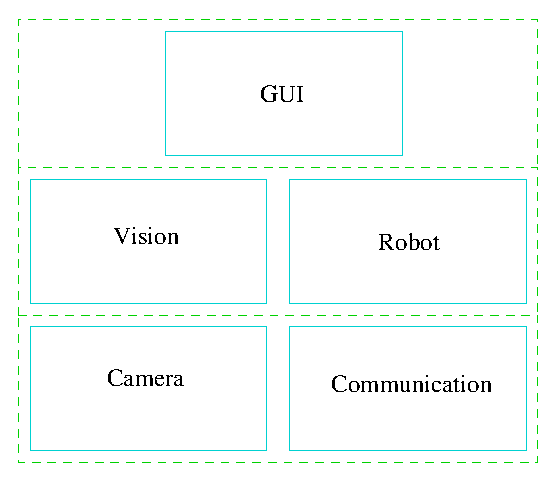
\includegraphics[width=5cm]{software-module}};}
    \uncover<3->{\node [below=0.1of right-image] {软件架构};}
  \end{tikzpicture}
\end{frame}

\begin{frame}{Design Example}
 \uncover<2->{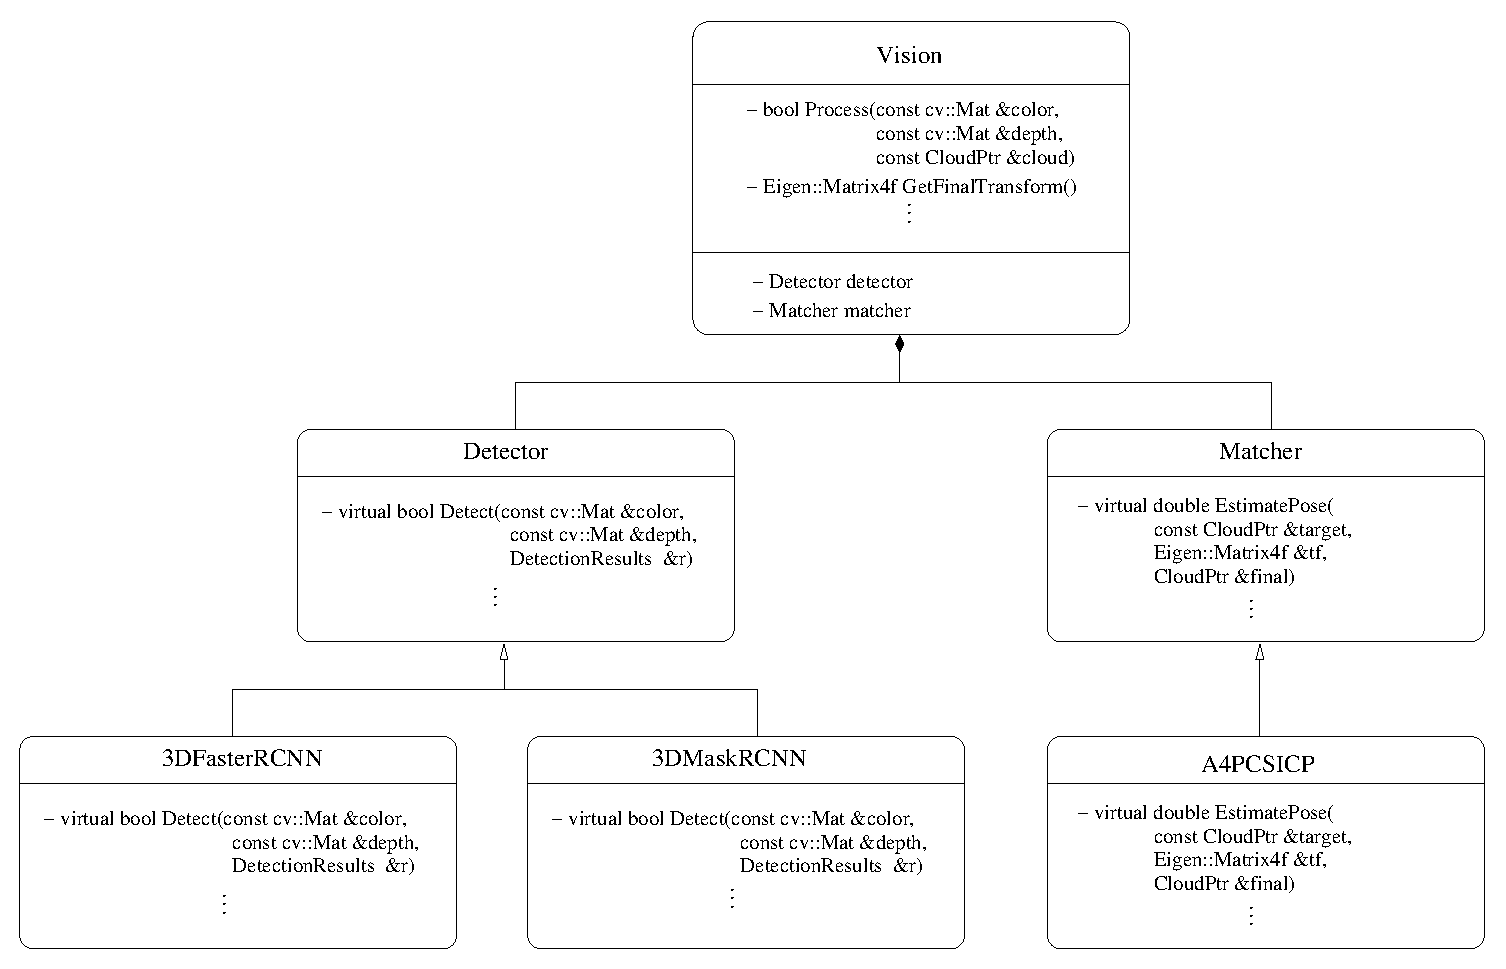
\includegraphics[width=10cm]{vision-uml}}
\end{frame}

\begin{frame}{Experiment}
  \begin{center}
    \begin{tikzpicture}
      \uncover<2->{
        \node (env) {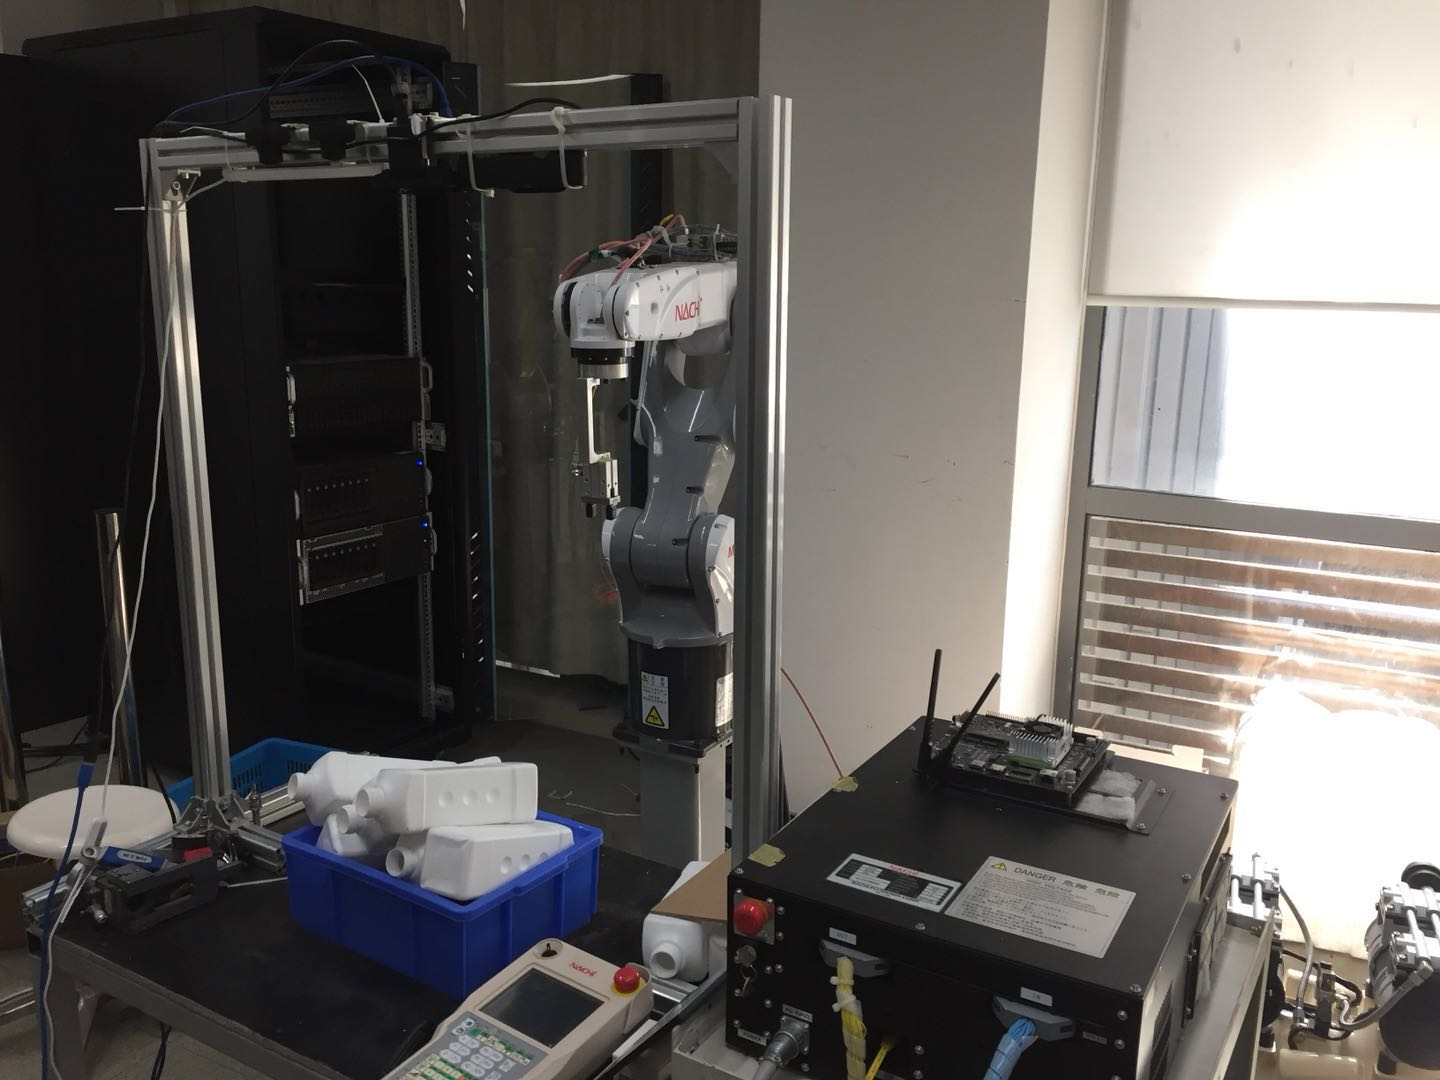
\includegraphics[width=5cm]{bin-picking-env}};
        \node[below =0.1 of env,font={\small}] {实验环境};
      }
      \uncover<3->{
        \node[right=0.2 of env] (box) {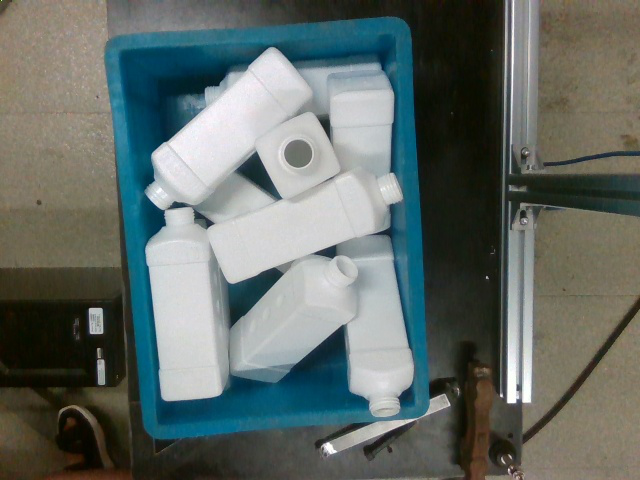
\includegraphics[width=5cm]{bin-picking-box}};
        \node[below =0.1 of box,font={\small}] {物料箱};
      }
    \end{tikzpicture}
  \end{center}
\end{frame}


\begin{frame}{Experiment \& Results}
  \begin{center}
  \uncover<2->{
  \resizebox{10cm}{!}{
  \begin{tabular}{cccccc}
    \toprule
    &成功率R&响应时间$T_r$&抓取时间$T_1$&放置时间$T_2$&工作周期$T$ \\
    \midrule
    1&100\%&711ms&7.6s&4.2s&11.9s \\
    2&100\%&729ms&6.8s&4.2s&11.0s \\
    3&100\%&708ms&6.5s&4.2s&10.7s \\
    4&100\%&701ms&8.1s&4.2s&12.3s \\
    5&100\%&713ms&9.3s&4.2s&13.5s \\
    6&100\%&722ms&6.6s&4.2s&10.8s \\
    7&100\%&693ms&7.9s&4.2s&12.1s \\
    8&100\%&732ms&9.1s&4.2s&13.3s \\
    9&100\%&718ms&8.9s&4.2s&13.1s \\
   10&100\%&723ms&6.9s&4.2s&11.1s \\
    \bf{Avg.}&\bf{100\%}&\bf{715ms}&\bf{7.77s}&\bf{4.20s}&\bf{11.98s} \\
    \bottomrule
  \end{tabular}
  }
  }
  \vfill
  \uncover<3->{
    \begin{equation*}
      T = T_1 + \max(T_r,T_2)
    \end{equation*}
  }
  \end{center}
\end{frame}

\begin{frame}{Experiment \& Results}
\begin{figure}[ht]
  \centering
  \subfloat[抓取成功率]{
    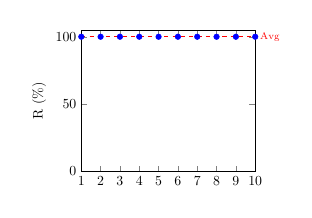
\begin{tikzpicture}[scale=0.5]
      \begin{axis}[
        width=6cm,
        ylabel=R (\%),
        xmin=1,xmax=10, xtick distance=1,
        ymin=0, ymax=105,
        clip=false
        ]
        \addplot[only marks, mark=*, blue] plot coordinates {
          (1,100)
          (2,100)
          (3,100)
          (4,100)
          (5,100)
          (6,100)
          (7,100)
          (8,100)
          (9,100)
          (10,100)
        };
        \addplot[red, dashed] plot coordinates {
          (1,100)
          (10,100)
        };
        \node[red,right] at (axis cs: 10,100) {\scriptsize{Avg}};
      \end{axis}
    \end{tikzpicture}
  }
  \hskip0.2cm
  \subfloat[响应时间]{
    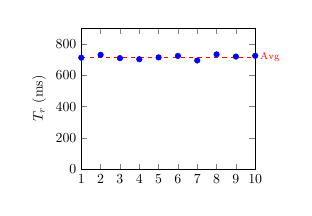
\begin{tikzpicture}[scale=0.5]
      \begin{axis}[
        width=6cm,
        ylabel=$T_r$ (ms),
        xmin=1,xmax=10, xtick distance=1,
        ymin=0, ymax=900,
        clip=false
        ]
        \addplot[only marks, mark=*, blue] plot coordinates {
          (1,711)
          (2,729)
          (3,708)
          (4,701)
          (5,713)
          (6,722)
          (7,693)
          (8,732)
          (9,718)
          (10,723)
        };
        \addplot[red, dashed] plot coordinates {
          (1,715)
          (10,715)
        };
        \node[red,right] at (axis cs: 10,715) {\scriptsize{Avg}};
      \end{axis}
    \end{tikzpicture}
  }
  \vfill
  \subfloat[抓取时间]{
    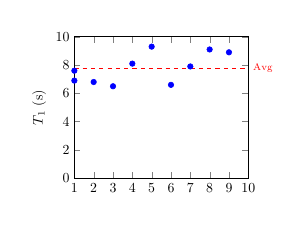
\begin{tikzpicture}[scale=0.5]
      \begin{axis}[
        width=6cm,
        ylabel=$T_1$ (s),
        xmin=1,xmax=10, xtick distance=1,
        ymin=0, ymax=10,
        clip=false
        ]
        \addplot[only marks, mark=*, blue] plot coordinates {
          (1,7.6)
          (2,6.8)
          (3,6.5)
          (4,8.1)
          (5,9.3)
          (6,6.6)
          (7,7.9)
          (8,9.1)
          (9,8.9)
          (1,6.9)
        };
        \addplot[red, dashed] plot coordinates {
          (1,7.77)
          (10,7.77)
        };
        \node[red,right] at (axis cs: 10,7.77) {\scriptsize{Avg}};
      \end{axis}
    \end{tikzpicture}
  }
  \hskip0.2cm
  \subfloat[放置时间]{
    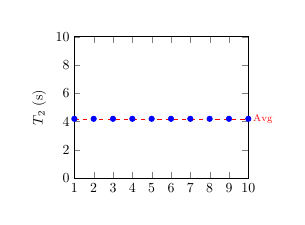
\begin{tikzpicture}[scale=0.5]
      \begin{axis}[
        width=6cm,
        ylabel=$T_2$ (s),
        xmin=1,xmax=10, xtick distance=1,
        ymin=0, ymax=10,
        clip=false
        ]
        \addplot[only marks, mark=*, blue] plot coordinates {
          (1,4.2)
          (2,4.2)
          (3,4.2)
          (4,4.2)
          (5,4.2)
          (6,4.2)
          (7,4.2)
          (8,4.2)
          (9,4.2)
          (10,4.2)
        };
        \addplot[red, dashed] plot coordinates {
          (1,4.2)
          (10,4.2)
        };
        \node[red,right] at (axis cs: 10,4.2) {\scriptsize{Avg}};
      \end{axis}
    \end{tikzpicture}
  }
  \hskip0.2cm
  \subfloat[工作周期]{
    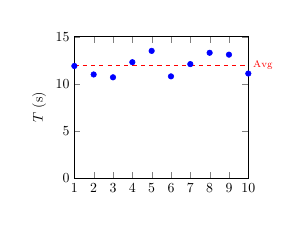
\begin{tikzpicture}[scale=0.5]
      \begin{axis}[
        width=6cm,
        ylabel=$T$ (s),
        xmin=1,xmax=10, xtick distance=1,
        ymin=0, ymax=15,
        clip=false
        ]
        \addplot[only marks, mark=*, blue] plot coordinates {
          (1,11.9)
          (2,11.0)
          (3,10.7)
          (4,12.3)
          (5,13.5)
          (6,10.8)
          (7,12.1)
          (8,13.3)
          (9,13.1)
          (10,11.1)
        };
        \addplot[red, dashed] plot coordinates {
          (1,11.98)
          (10,11.98)
        };
        \node[red,right] at (axis cs: 10,11.98) {\scriptsize{Avg}};
      \end{axis}
    \end{tikzpicture}
  }
  \label{fig:app_res}
\end{figure}
  
\end{frame}
\section{Conclusion}

\begin{frame}{Summary}
  \begin{itemize}
  \item<2-> 对偶RGB-D相机结构相比单个RGB-D相机有更高的填充率,更低的噪声,但对精度的提升不明显
  \item<3-> 3D-MRAI算法相比传统算法表现出了较高的检测准确率,估计的位姿精度也更高,但FPS较低
  \item<4-> 基于3D-MRAI算法设计的Bin-Picking视觉系统具有更高的抓取成功率、更快的响应速度,以及更低的成本
  \end{itemize}
\end{frame}

{\setbeamercolor{palette primary}{fg=black, bg=yellow}
\begin{frame}[standout]
  \hyperlink{contents}{{Questions?}}
\end{frame}
}

\appendix

% \begin{frame}[fragile]{Backup slides}
  % \tableofcontents
% \end{frame}

% \begin{frame}[allowframebreaks]{References}

%   \bibliography{demo}
%   \bibliographystyle{abbrv}

% \end{frame}

\end{document}

%%% Local Variables:
%%% mode: latex
%%% TeX-master: t
%%% End:
